\documentclass[a4paper, 16pt]{article}
\usepackage[slovene]{babel}
\usepackage[utf8]{inputenc}
\usepackage[T1]{fontenc}
\usepackage{lmodern}
\usepackage{hyperref}
\usepackage{graphicx}
\usepackage{wrapfig}

\title{Analiza BlackJack strategij \\ Poročilo}
\date{Maj 2022}
\author{Zala Stopar Špringer}


\begin{document}

\maketitle

\section{Kratek opis}

Za projekt pri predmetu Matematika z računalnikom sem raziskovala različne strategije stavljanja. Svoj program sem napisala v programskem jeziku \textit{Python}. Aplikacijo sem oblikovala s pomočjo paketa \textit{Pygame}. Glavni del igre je napisan v datoteki \textbf{gaming.py}\\

\noindent Na začetku sem se lotila programiranja in dizajniranja navadne igre BlackJack, ki sem jo tudi dokončala. Posameznik se lahko pomeri proti hiši. Skupaj je v igri 6 kompletov kart. Na vsakem koraku ima igralec na voljo akciji HIT in STAND, v pravih okoliščinah pa tudi INSURANCE, DOUBLE DOWN in SPLIT. V različih igralnicah se pravila malo razlikujejo. Za moj program sem določila, da po tem, ko igralec izbere opcijo SPLIT, nima več na voljo opciji DOUBLE in INSURANCE. \\


\noindent Opazovala sem rezultate sledečih strategij:
\begin{itemize}
\item Paroli system
\item 1 3 2 6 system
\item Reverse Labouchere
\item Card counting
\item Martingale
\item Oscar’s Grind
\item Labouchere
\end{itemize}
Te so zbrane v mapi \textbf{functions} v datoteki \textbf{strategies.py}, njihov opis pa sledi kasneje v poročilu.

\section{Opis strategij}

\subsection{Paroli system}
Kot pri večini strategij, je tudi pri Paroli sistemu potrebno določiti enoto stavljanja. Pri tem sistemu spreminjamo stavo glede na število zaporednih iger, ki smo jih zmagali. Po zmagi, se stava v naslednji igri podvoji. V mojem primeru sem stavo podvojevala do treh zaporednih zmag, nato pa sem se vrnila na zaćetno enoto. Seveda je lahko meja števila zaporednih zmag, ko se vrnemo na začetno stavo višja, je pa zato taka igra tudi bolj tvegana.

\subsection{1 3 2 6 System}
Tudi 1326 sistem spreminja velikost stave glede na število zaporednih zmag. Po zmagi, velikost stave v naslednji igri znaša \textit{enota} $\times 3$, po dveh zaporednih stavah v naslednji igri stavimo \textit{enota} $\times 2$ in po treh zaporednih zmagah stavimo \textit{enota} $\times 6$. Nato se vrnemo na začetek in postopek ponovimo. Od tod izvira ime $1326$. Seveda se vrenmo nazaj na prvotno enoto, če zadnjo igro izgubimo.

\subsection{Reverse Labouchere}
Pri tej strategiji začnemo z oblikovanjem zaporedja številk, katerih vsota se mora sešteti v zaželjen dobiček. Za prvo stavo seštejemo prvo in zadnjo število v zaporedju. Če mešanje zmagamo, vsoto dodamo na konec našega zaporedja, sicer pa števili odstranimo iz seznama. nato zopet stavimo vsoto prvega in zadnjega števila. Ko (Če) je naše zaporedje prazno, smo zaslužili željeno vsoto.

\subsection{One half increase}
Podobno kot prvi dve strategiji, ta strategija spreminja stavo glede na število zaporednih zmag. Prav tako pa začnemo stavljati z eno enoto, ki je v naprej izbrana. Ko zmagamo dve mešanji zapored, povečamo stavo za polovico enote. To ponavljamo, dokler ne izgubimo mešanja. Takrat se vrnemo na prvotno enoto in ponovno začnemo cikel.

\subsection{Card counting}
Tako kot zgoraj opisane strategije,  deluje tudi ta glede na število zaporednih zmag. Pred začetkom igranja se vsaki karti določi svojo vrednost, v mojem primeru so karte v vrednosti od $2$ do $6$ znašale $+1$, karte $7, 8, 9$ so predstavljale vrednost 0, $10$ ali višje pa $-1$. Igralec po vsaki karti, ki pade na mizo spremeni štetje glede na vrednost karte. Ker igralnice igrajo ogro z večimi paketi kart, je treba vrednost štetja spremeniti, tako da ga delimo s številom preostalih paketov kart.  Višje, ko je štetje, višja je stava. V mojem primeru sem stavila osnovno enoto, če je bilo štetje $1$ ali manjše, sicer pa (\textit{štetje} - 1) $\times$ \textit{enota} $\times 10$. %%%%%%%% a je res x 10

\subsection{Martingale}
Pri tej strategiji se višina stae speminja glede na število zaporednih porazov. Po vsakem porazu, je stava v naslednji igri dvakrat večja. Ko prvič zmagamo, si povrnemo našo izgubu in nekaj malega pridobimo. Seveda pa stave lahko zelo hitro narastejo, zato je čim bolje začeti z minimalno stavo, da imamo možnost zmagati eno igro, preden nam zmanjka denarja.

\subsection{Oscar's Grind}
Tudi ta strategija deluje na podlagi števila zaporednih izgubljenih iger. Dokler ne zmagamo stavljamo v višini ene enote. Ob zmagi stavimo edve enoti in stavljamo dokler ne zmagamo, nato stavimo 3 enote, \dots. Postopek ponavljamo, dokler skupno ne zaslužimo ene enote. Nato vse ponovimo.

\subsection{Labouchere} 
Ta strategija deluje zelo podobno kot Reverse Labouchere. Prav tako se začne z zaporedjem številk. Prva stava je enaka vsoti prve in zadnje številke v zaporedju. Če igro zmagamo, številki prečrtamo, sicer pa vsoto dodamo na konec seznama. Naslednja stava pa zopet znaša vsoto prve in zadnje številke. 

 \section{Oblikovanje vmesnika}

Pri tem projektu sem se prvič spoznala s knjižnjico \textit{Pygame}. Večina objektov v aplikaciji je sestavljena iz različnih kvadratov, z različnimi lastnostmi. Poleg tega si delo olajšala s tem, da sem ustvarila razred \textbf{Button}, ki mu podamo pozicijo, besedilo v gumbu, 3 različne barve, velikost in obrobo. Pri ustvarjanju razreda \textbf{InputBox} sem imela več težav. Zato sem si kodo izposodila iz spletne strani \href{https://stackoverflow.com/questions/46390231/how-can-i-create-a-text-input-box-with-pygame}{Stack Overflow}, dodala pa sem nekaj vrstic, ki sem jih potrebovala za svojo igro.\\

Ker sem se z omenjeno knjižnjico šele spoznavala, sem se za začetek lotila oblikovanja lažjih oken. Po tem, ko sem izbrala ustrezno bravno paleto sem oblikovala začetno stran igre, ki je shranjena v mapi \textbf{windows} pod imenom \textit{menu\_window.py}. Kot je vidno na sliki, imamo na uvodi strani na voljo nekaj možnosti, lahko igramo navadno igro, lahko igramo igro s pomočjo ali pa simuliramo igro. 


\begin{figure}[htbp]
\centering
\setkeys{Gin}{width=0.45\linewidth}
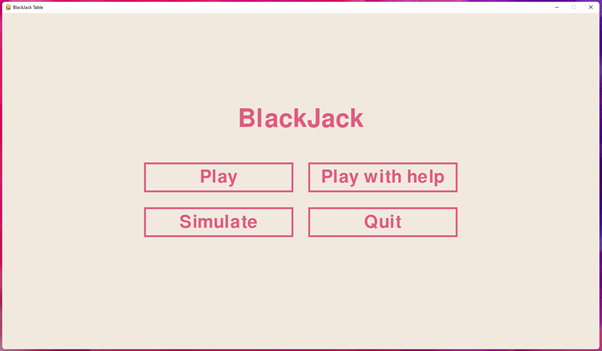
\includegraphics{meni.png}\,%
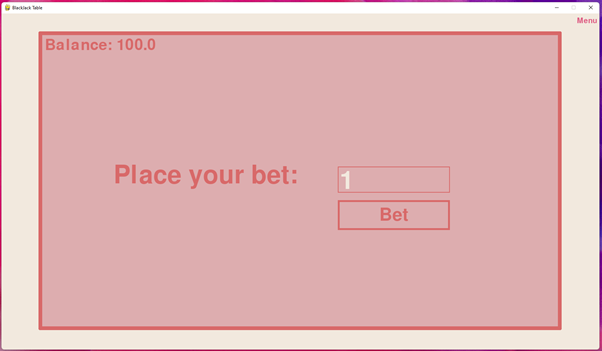
\includegraphics{bet.png}
\caption{Menu and Bet windows}
\label{fig:menu}
 \end{figure}


Ne glede na možnost, ki jo izberemo, nas aplikacija postavi na stran, kjer položimo vsoto, s katero bi radi igrali. V primeru navadne igre in igre s pomočjo se nato znajdemo na strani, kjer stavimo prvo stavo. To stran lahko tudi vidimo na sliki \ref{fig:menu}.V nasprotenm primeru se odpravimo na stran (izbira simulacije), kjer poleg vsote, s katero bi radi igrali izberemo tudi število igre, ki bi jih radi igrali in število mešanj v posamezni igri. Poleg tega izberemo tudi strategijo stavljanja, ki bi jo radi igrali in osnovno enoto stave.
Ko končamo z igranjem igre nas vrže na zaključno stran, kjer lahko prevzamemo dobitek. \\

% slika kart
Nekaj novih stvari sem se tudi nučila pri oblikovanju kart. Da nisem risala usake karte posebej, sem ustvarila razred po imenu \textbf{Card} s parametri brava, vrednost in pozicija karte. Z metodo \textit{.draw()} lahko karto narišemo, z metodo \textit{.card\_back()} pa narišemo hrbtno stran karte. Za sliko na hrbtni strani karte in za simbole barv sem poiskala ikone na spletni strani \url{https://www.flaticon.com/}.


% Strategije so opisane \href{https://www.legitgamblingsites.com/blog/how-to-best-take-advantage-of-streaks-in-blackjack/}{tukaj,}

\section{Še sledi}
\begin{itemize}
\item dokončati igro, kjer je navoljo pomoč
\item napisati funkcijo za računanje verjetnosti zmage v določeni situaciji
 \item dodati strategijo štetja kart
\item napisati funkcijo za hranjenje podatkov iz simulacije različnih strategij
\item analizirati dobljene podatke
\end{itemize}




\end{document}